\section{Включение/выключение робота}
Для включения робота нажмите и удерживайте кнопку~1 до тех пор пока индикаторный светодиод~2 не перестанет мигать.
После этого отпустите кнопку и дождитесь окончания загрузки.

\begin{figure}[h]
	\centering
	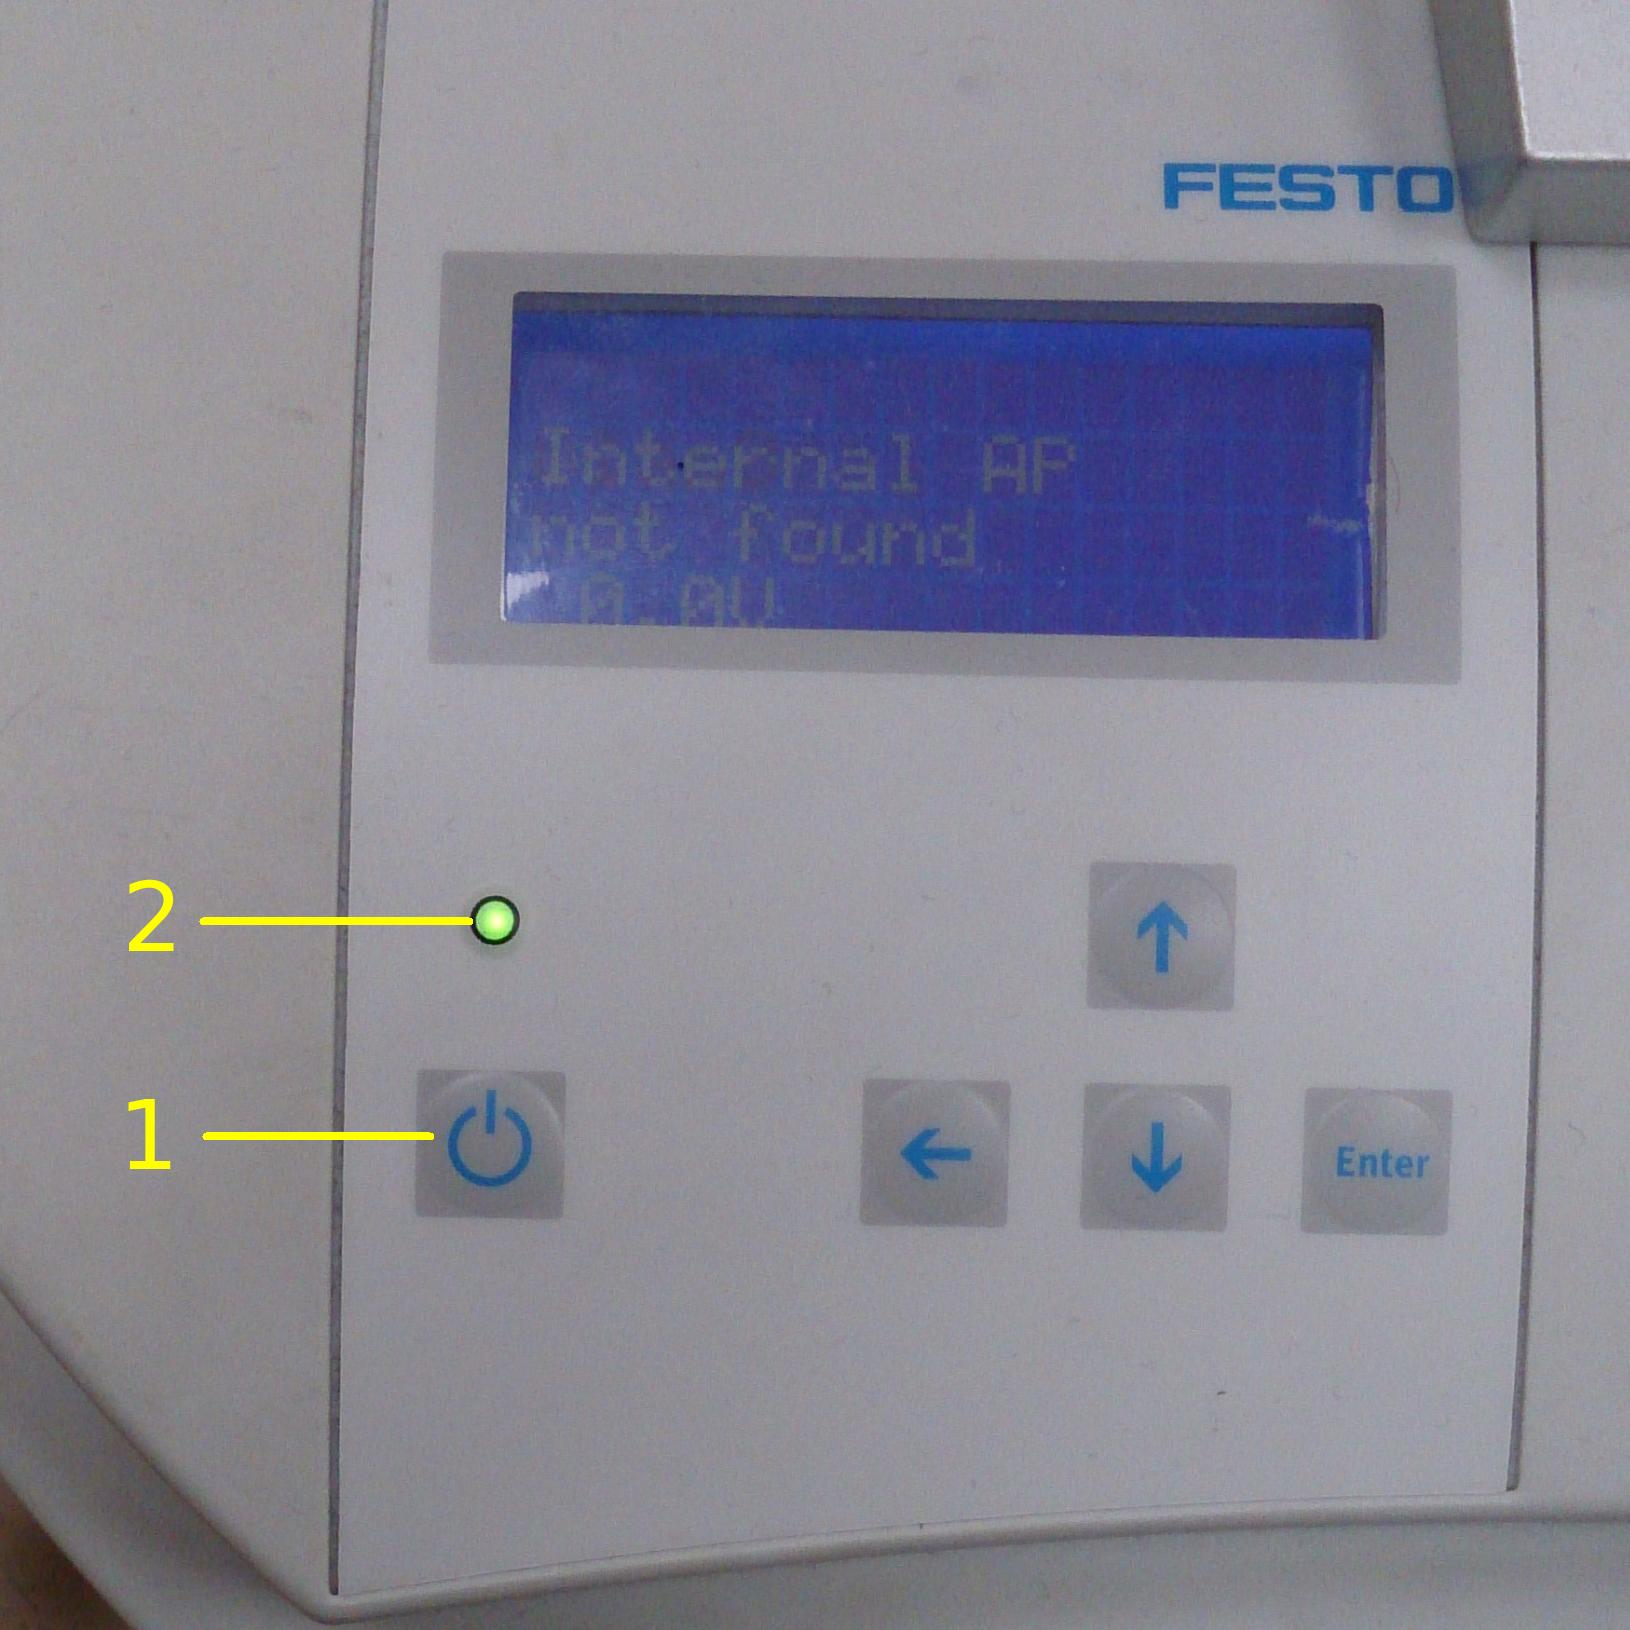
\includegraphics[width=0.4\textwidth]{interface.jpg}
	\caption{Кнопочно-дисплейный интерфейс Robotino.}
	\label{img_interface}
\end{figure}

Стоит отметить, что на определенном этапе загрузки робот может самостоятельно отключиться.
В этом случае просто включите его еще раз.
Если такое его поведение повторится более двух раз, попробуйте заменить ему батареи или поставить его на зарядку.

Для выключения робота нажмите и удерживайте кнопку~1 до тех пор пока индикаторный светодиод, перестав мигать, не потухнет.
После этого отпустите кнопку.



\newpage
\section{Зарядка робота}\label{part_charging}
Для зарядки пары аккумуляторов, установленных на робота, воткните штекер зарядного устройства в вилку, торчащую с левого борта Robotino (см.~рисунок~\ref{img_charging_of_robot}).

Для зарядки пары аккумуляторов, не установленных на робота, соедините их перемычкой и подключите свободные полюса к зарядному устройству с помощью «переходника», оснащенного зажимами-крокодилами (см.~рисунок~\ref{img_charging_of_batteries}).

Если понадобится произвести замену аккумуляторов на Robotino, отверните четыре показанные на рисунке~\ref{img_remove_head} винта и аккуратно снимите командный блок (<<голову>>) робота.
После этого снимите вилки (или зажимы-крокодилы) с клемм старых аккумуляторов, а также прижимную планку, фиксирующую аккумулятор на месте его установки, освободив ее концы от прижимных петель (см.~рисунок~\ref{img_remove_accum}).
После этого замените старые аккумуляторы на новые и повторите все указанные действия в обратном порядке.
Будьте осторожны при установке на место командного блока робота по той причине, что можно повредить разъемы его электрического соединения с несущей платформой!

\begin{figure}[h!]
    \centering
    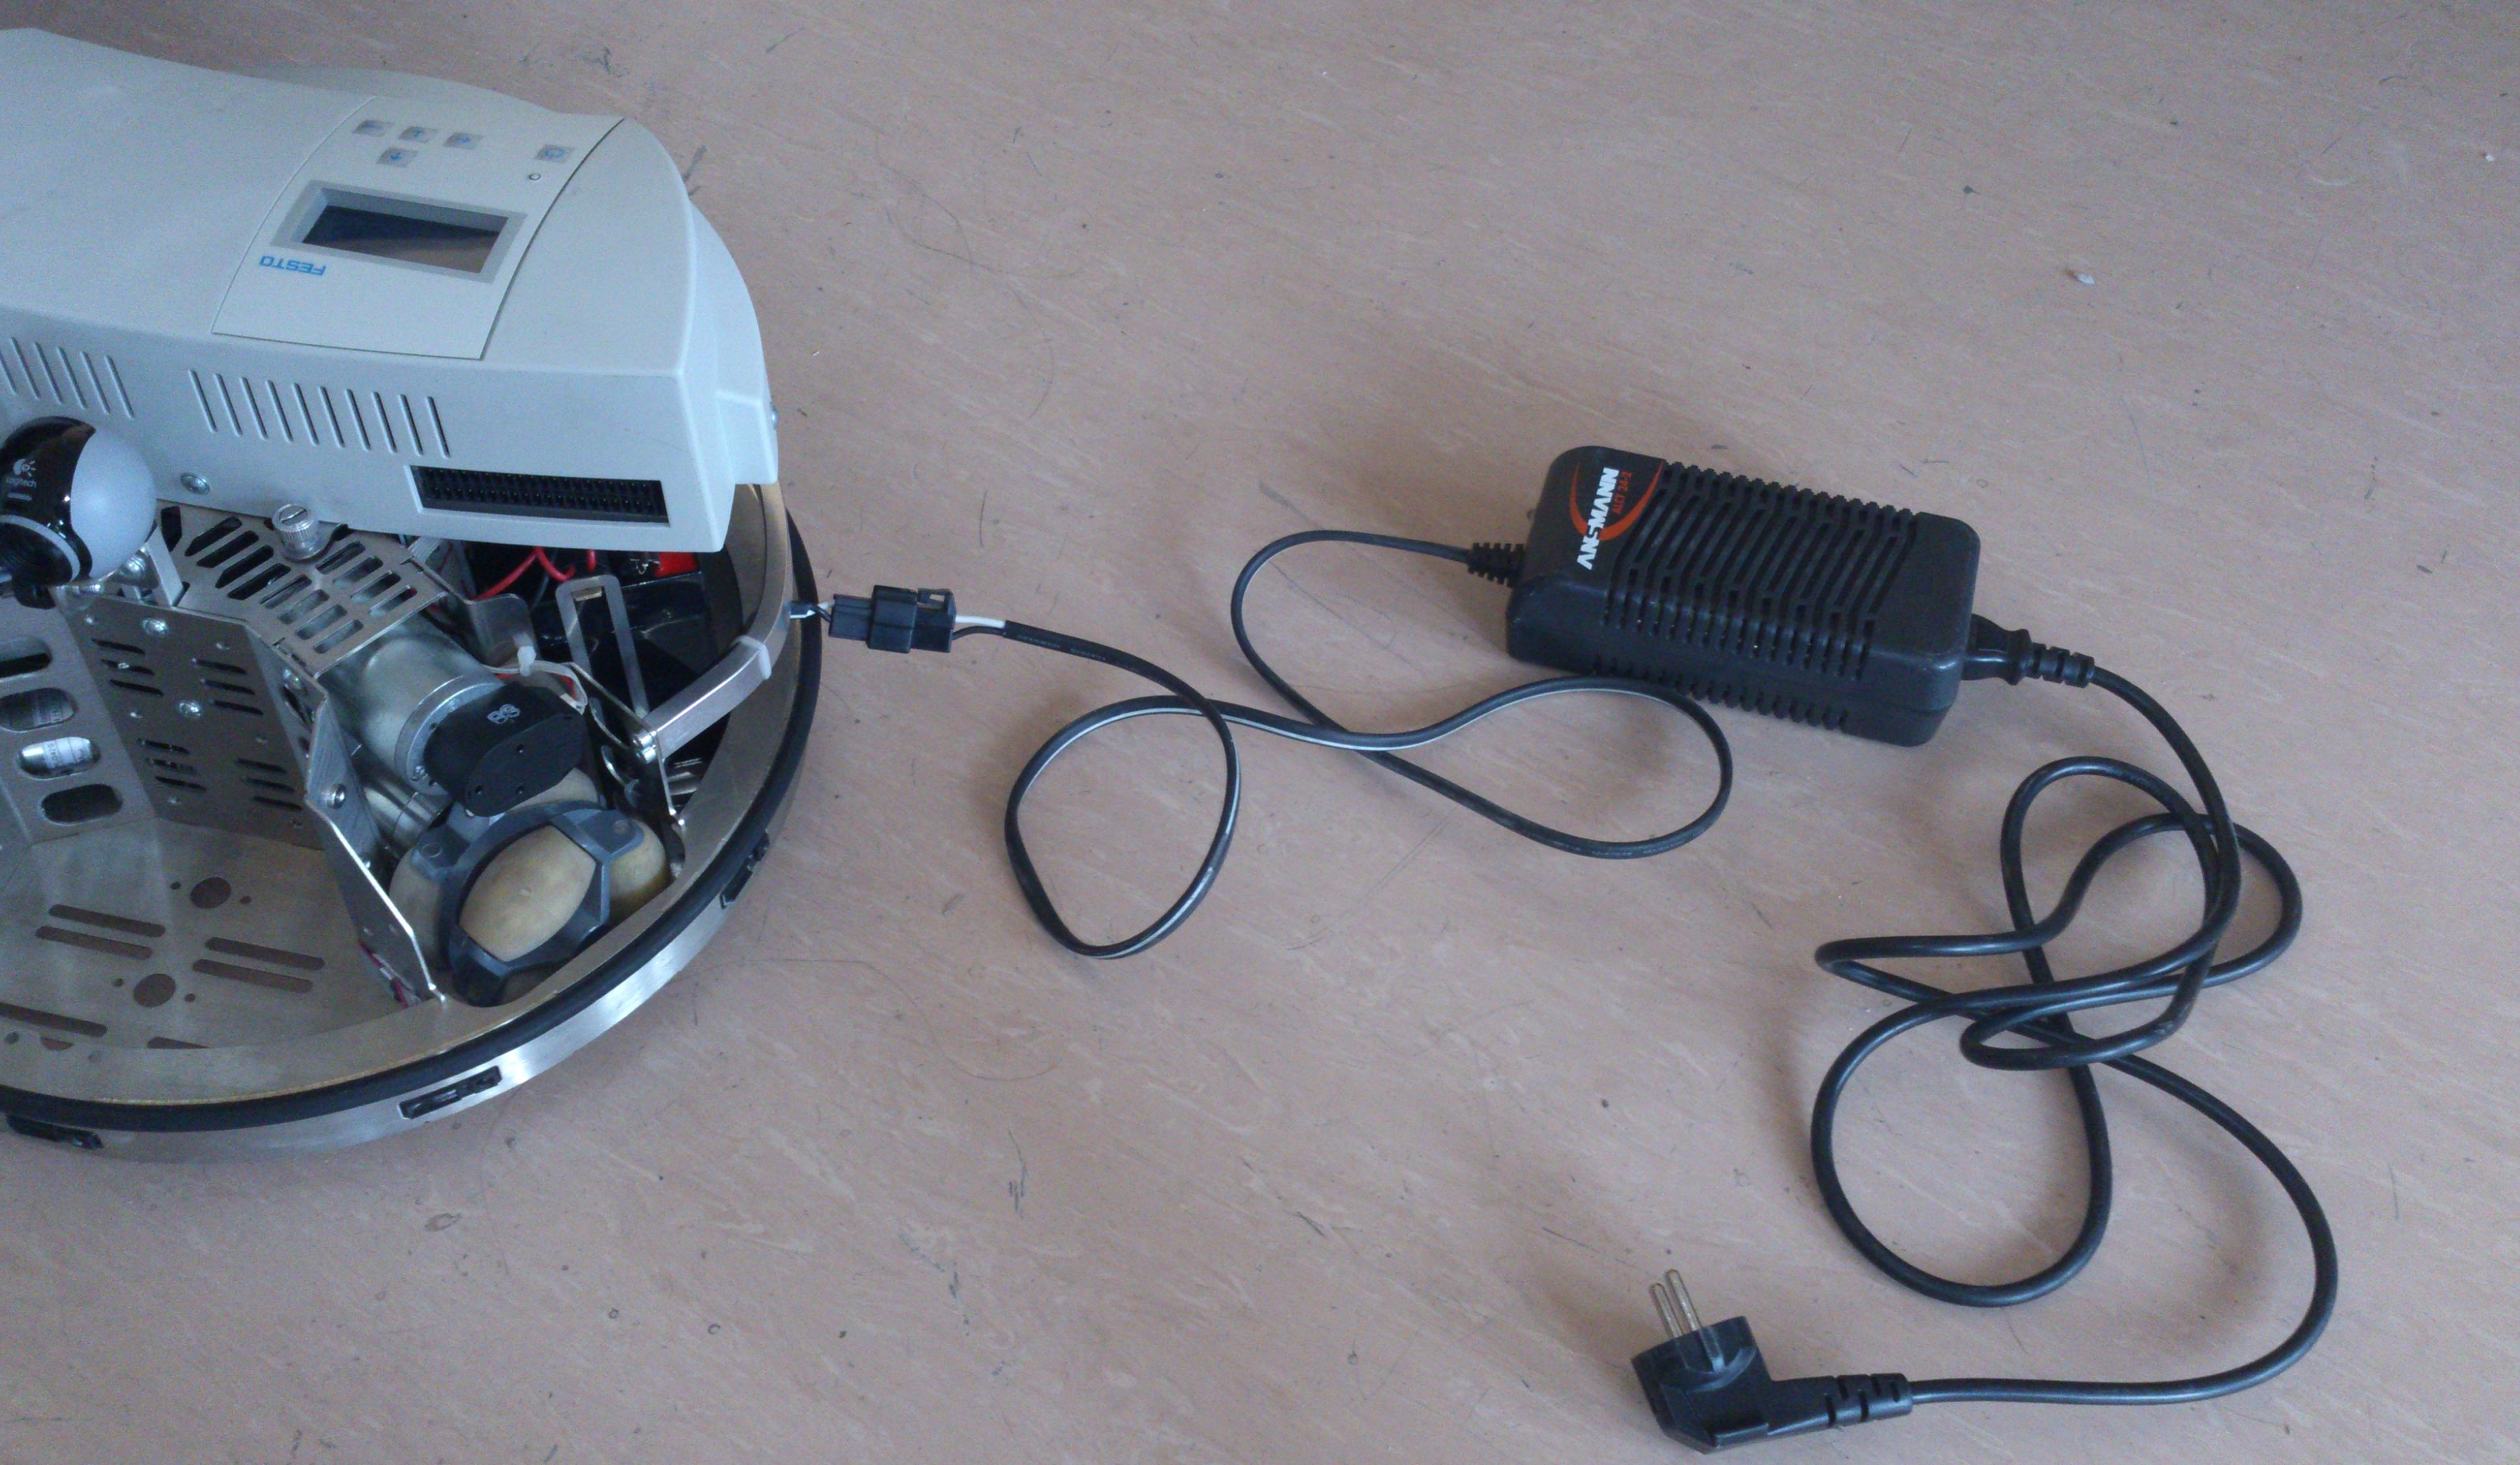
\includegraphics[height = 7.5cm]{charging_of_robot.jpg}
    \caption{Зарядка аккумуляторов, установленных на робота.}
	\label{img_charging_of_robot}
\end{figure}

\begin{figure}[h!]
	\centering
	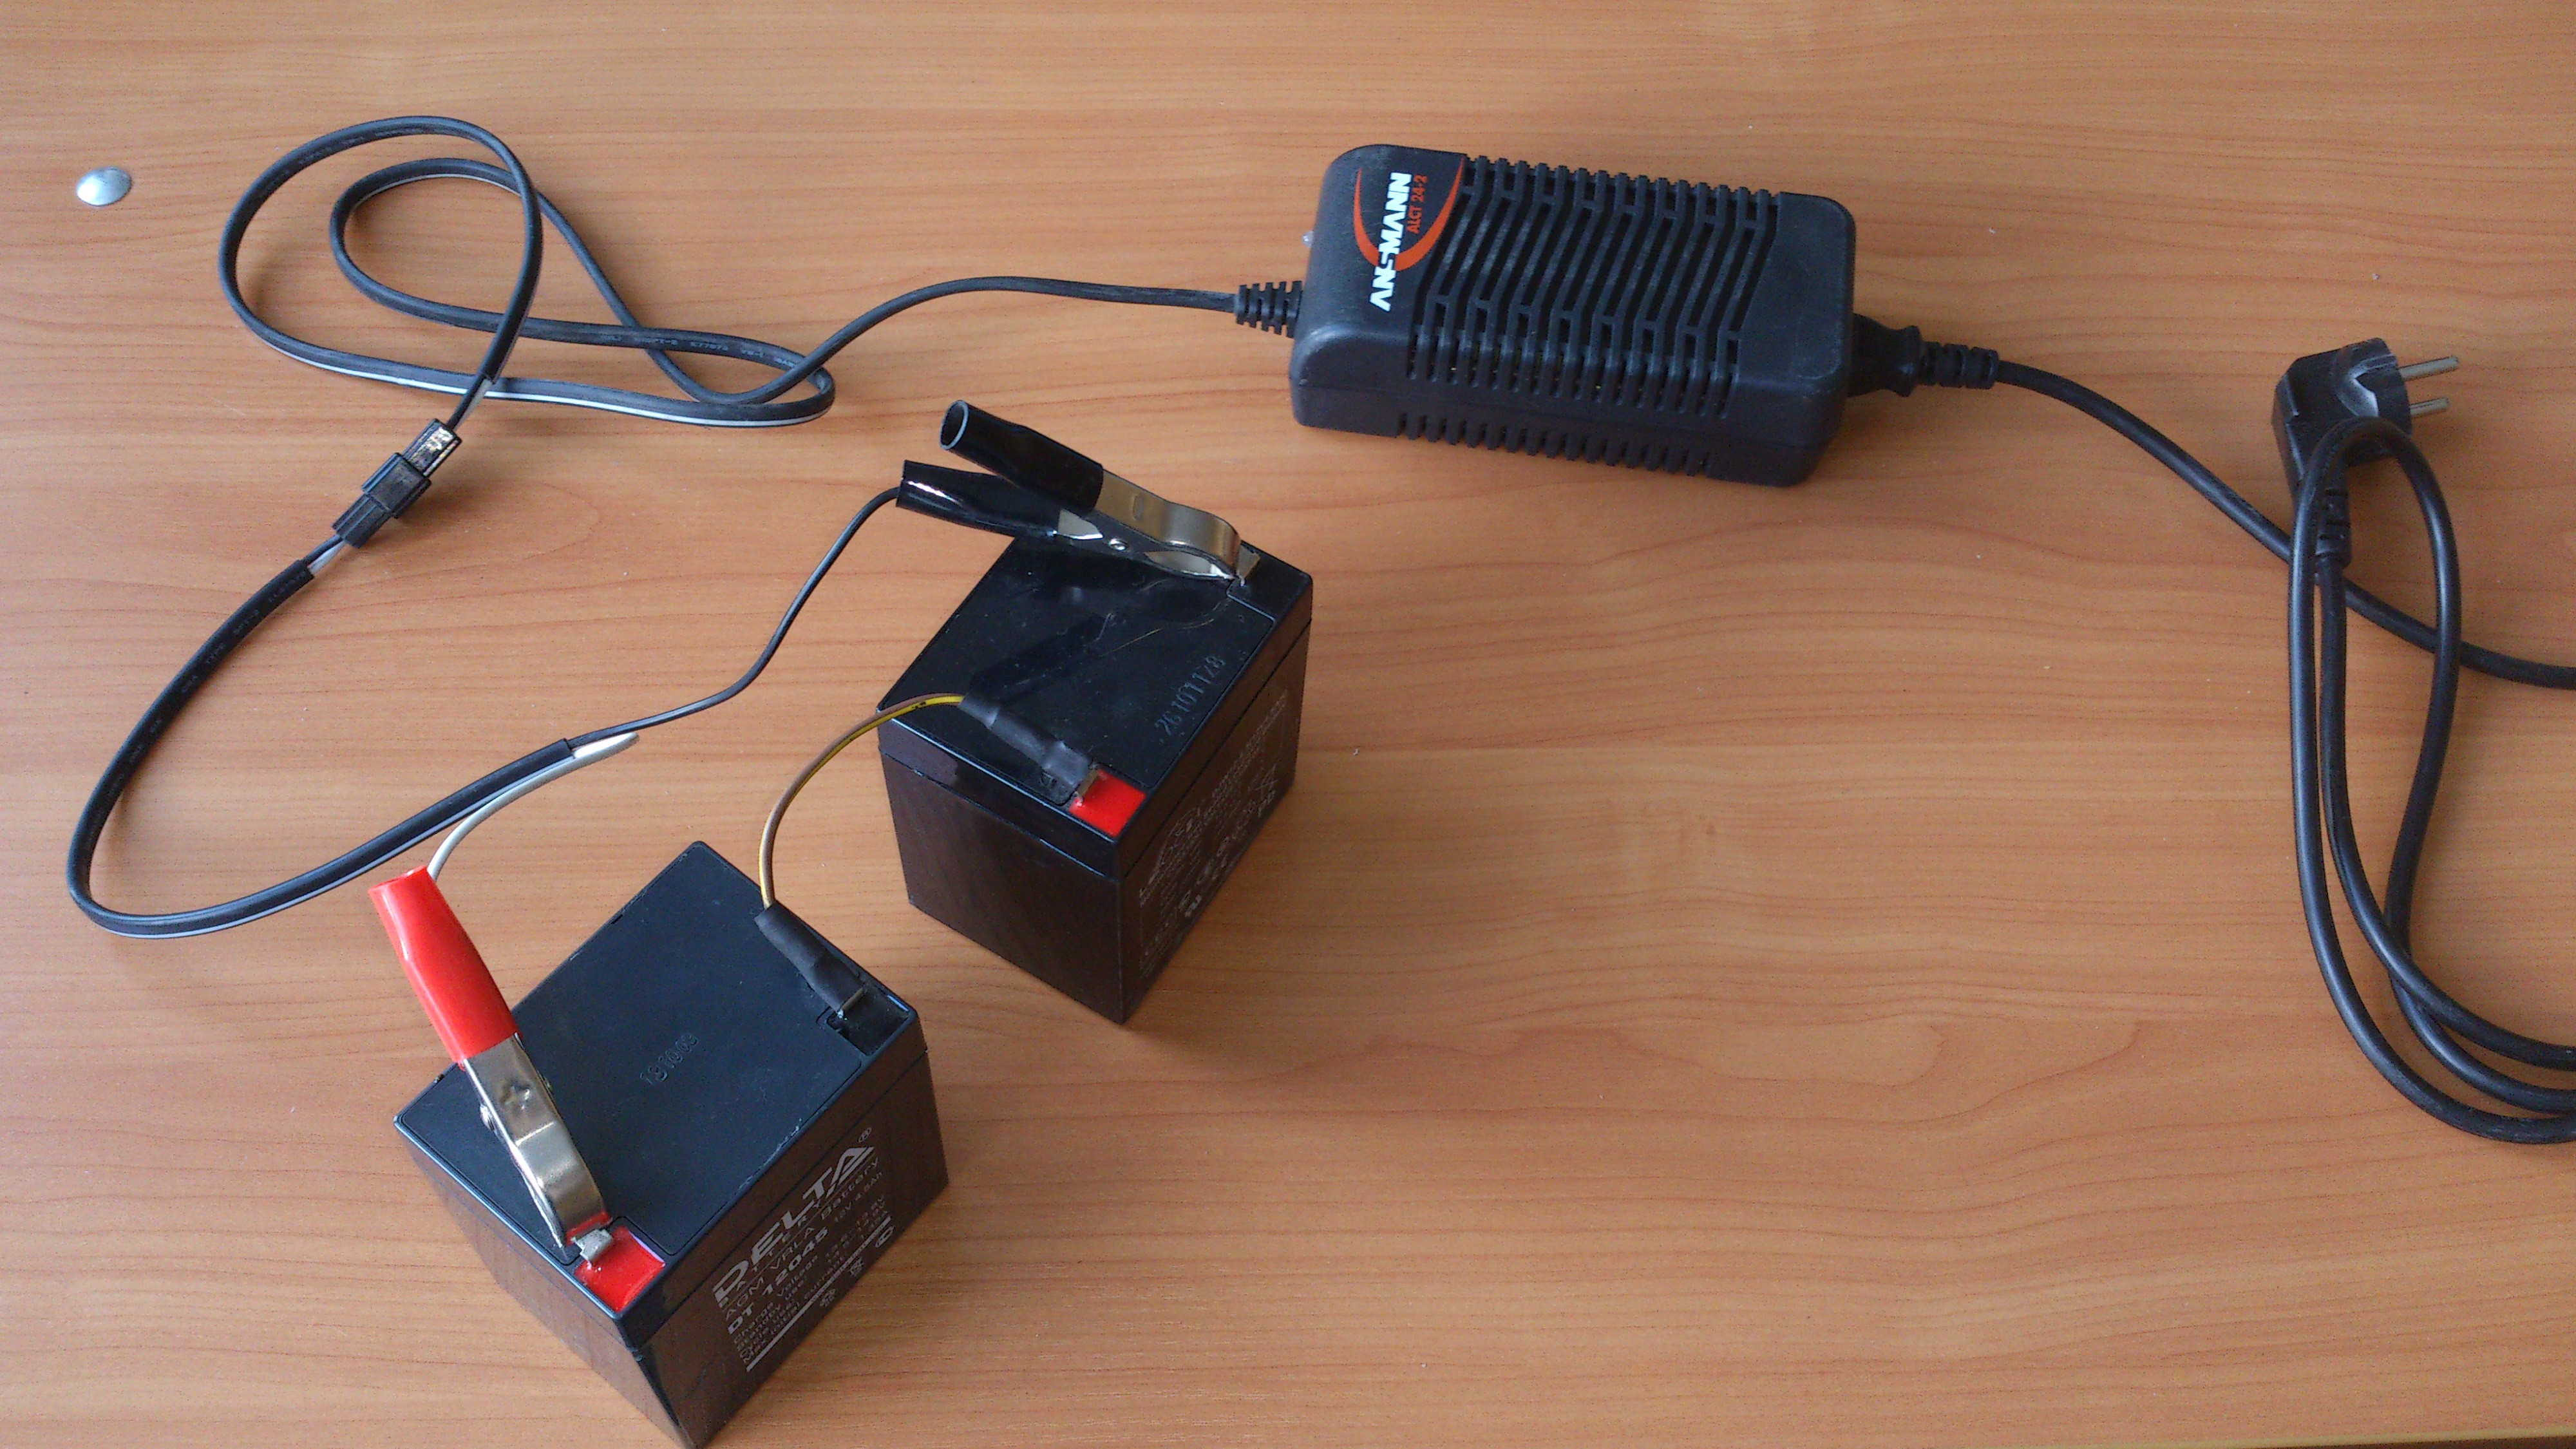
\includegraphics[height = 7.5cm]{charging_of_accums.jpg}
	\caption{Зарядка отдельно стоящих аккумуляторов.}
	\label{img_charging_of_batteries}
\end{figure}

\begin{figure}[p]
	\begin{minipage}[h]{0.55\linewidth}
		\centering{ 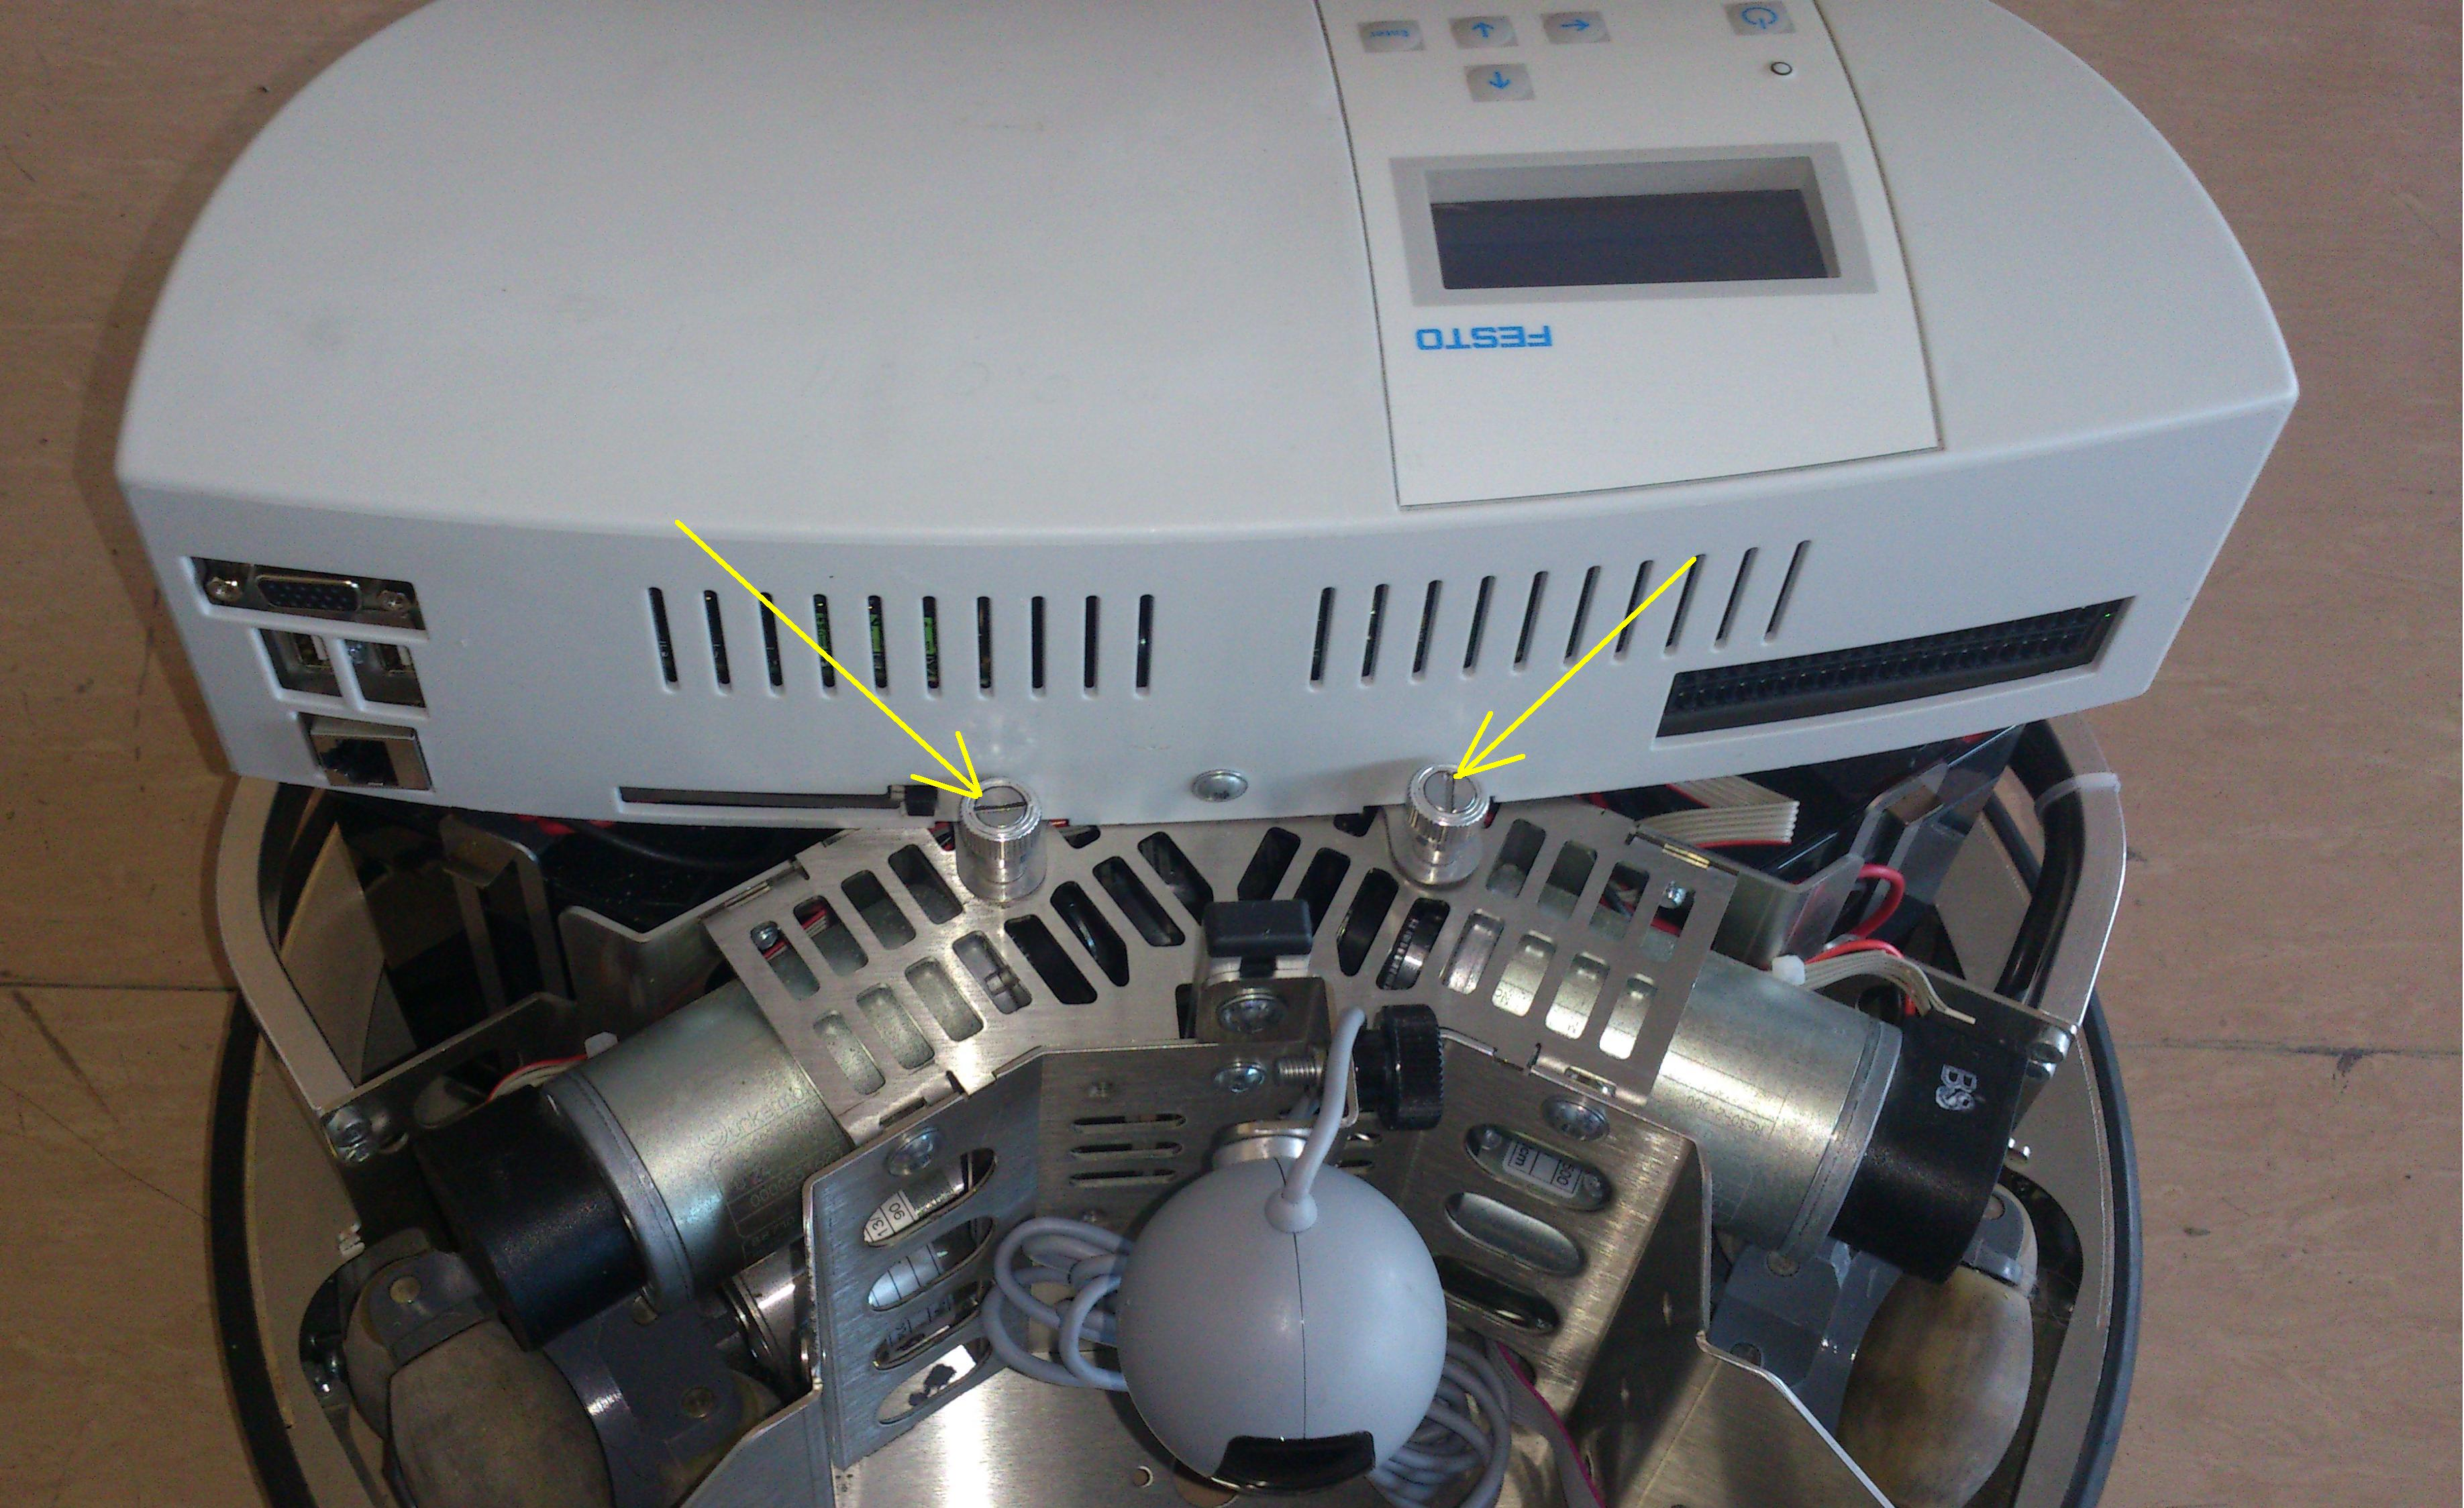
\includegraphics[height = 5.9cm]{remove_head1.jpg} }
	\end{minipage}
	\hfill
	\begin{minipage}[h]{0.44\linewidth}
		\centering{ 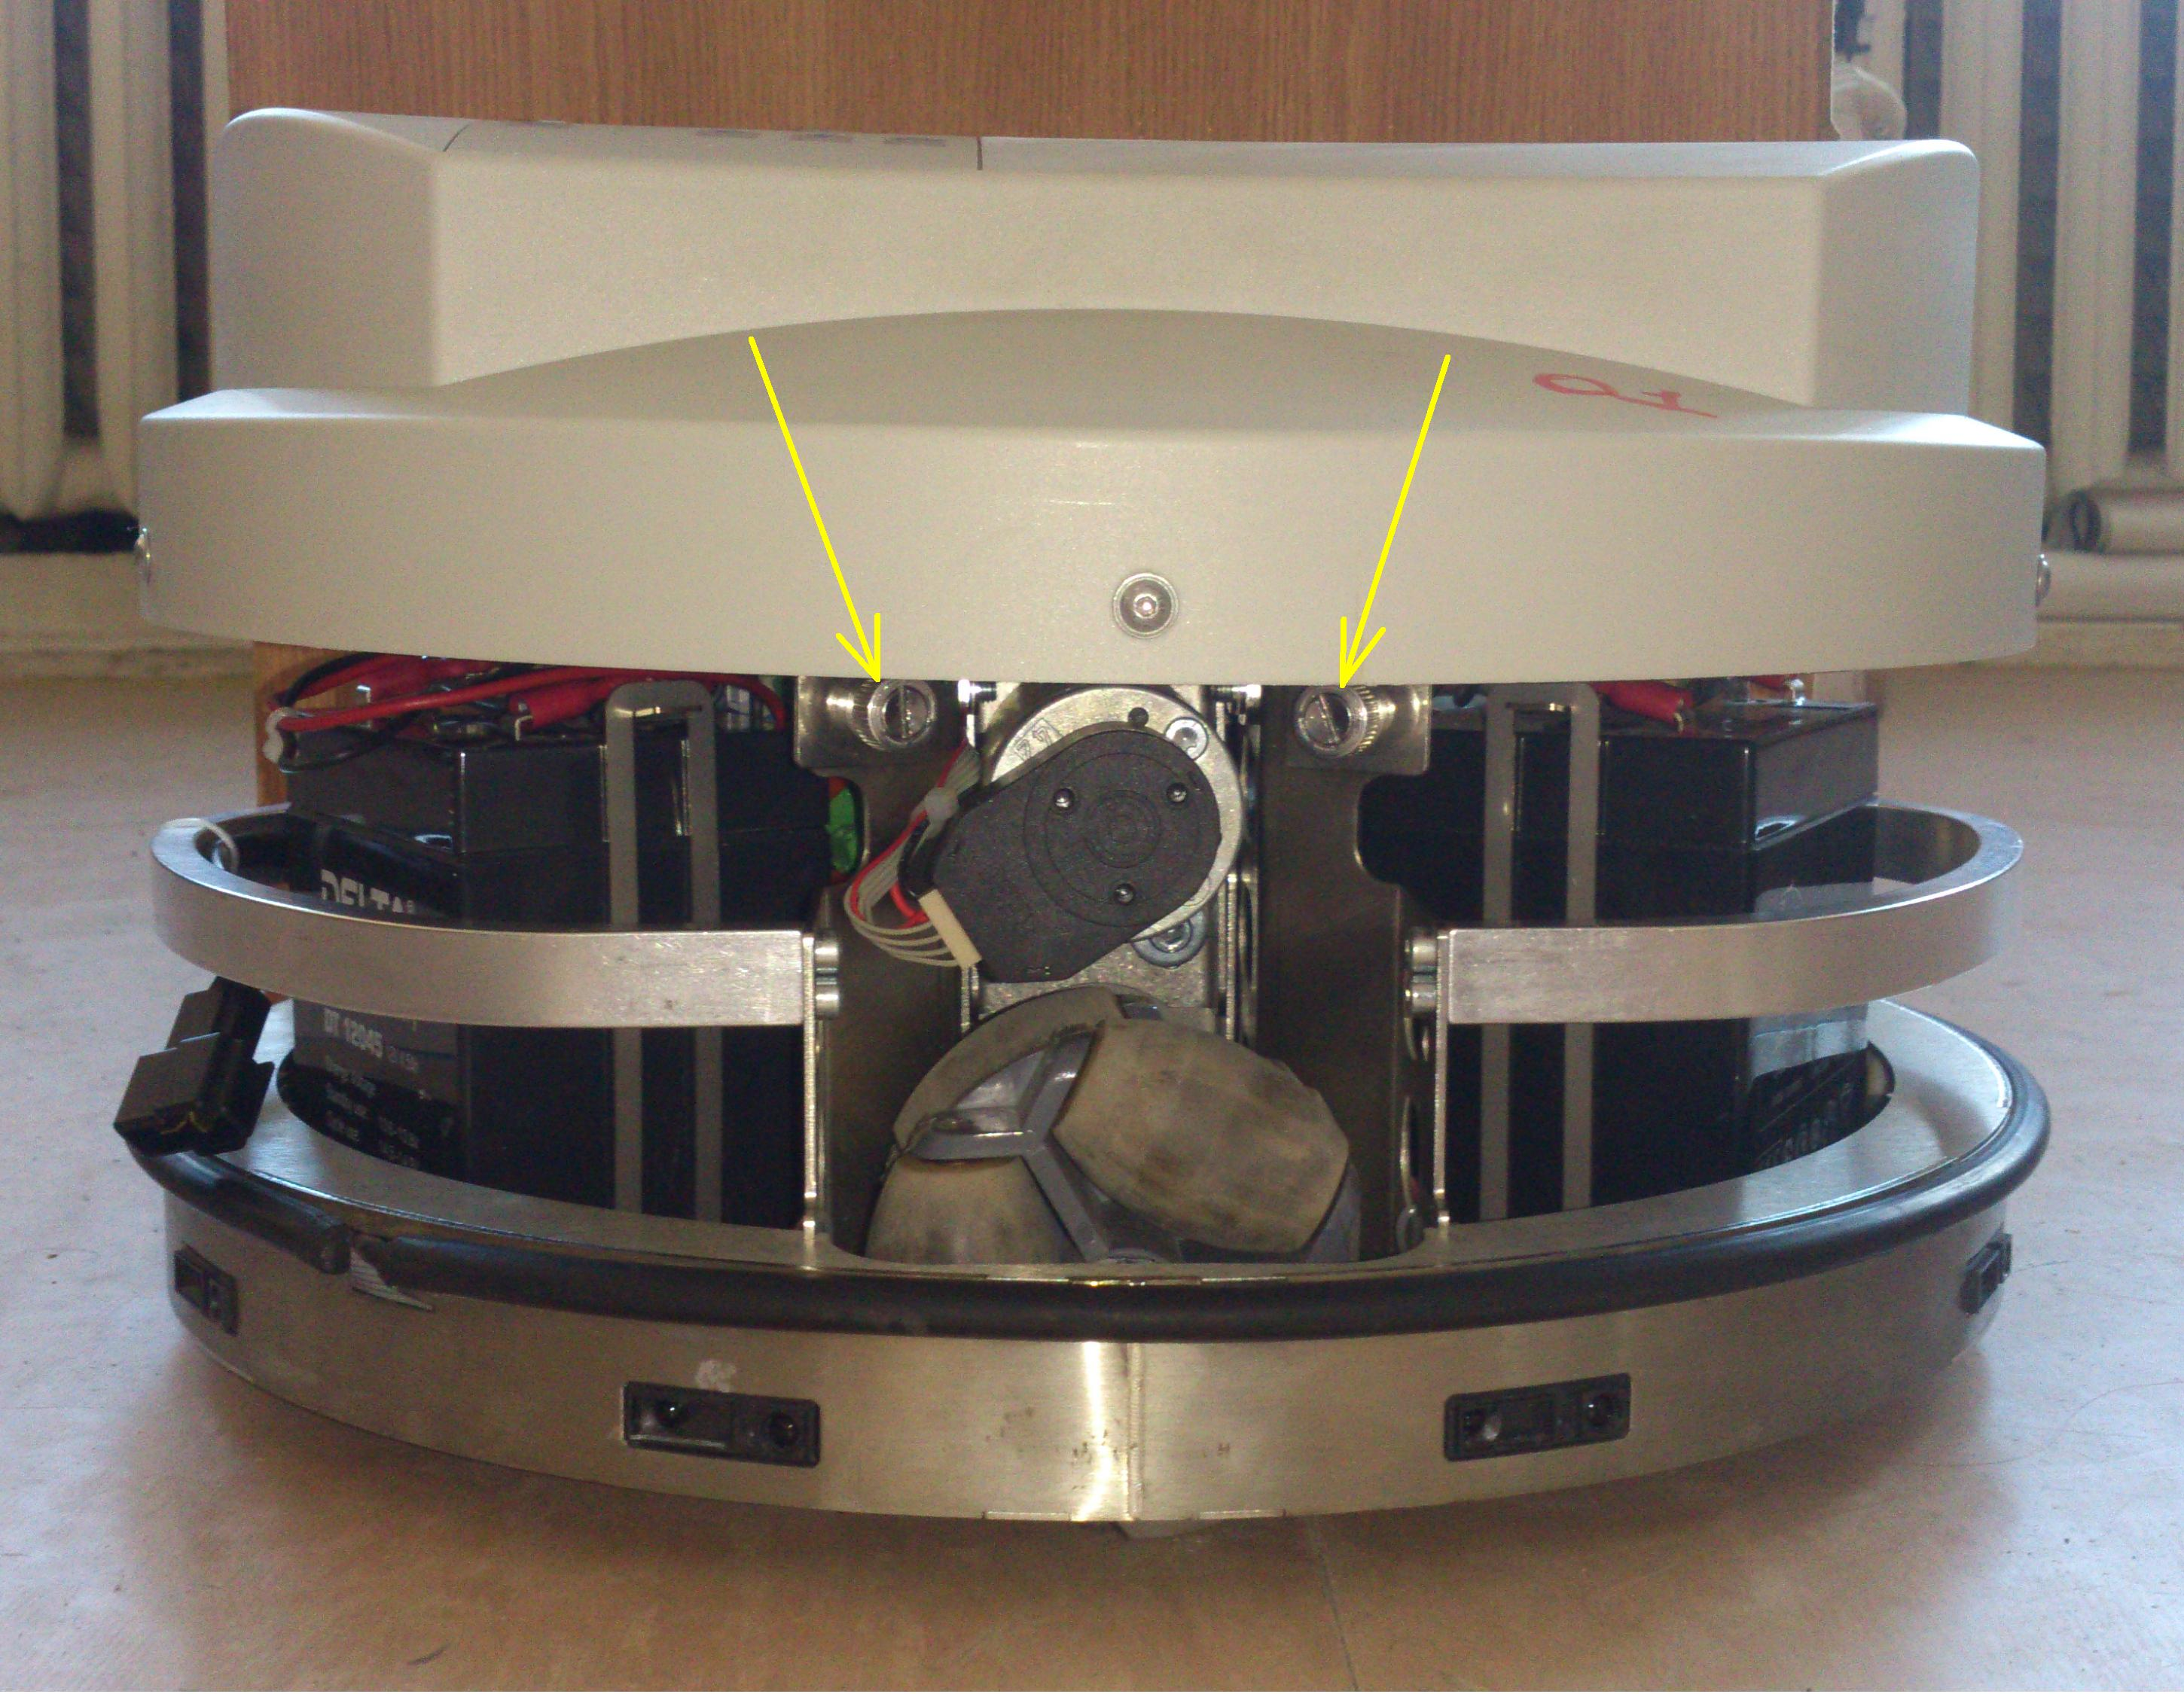
\includegraphics[height = 5.9cm]{remove_head2.jpg} }
	\end{minipage}
	\caption{Винты, соединяющие <<голову>> и колесную базу робота.}
	\label{img_remove_head}
\end{figure}

\begin{figure}[p]
	\begin{minipage}[h]{0.49\linewidth}
		\centering{ 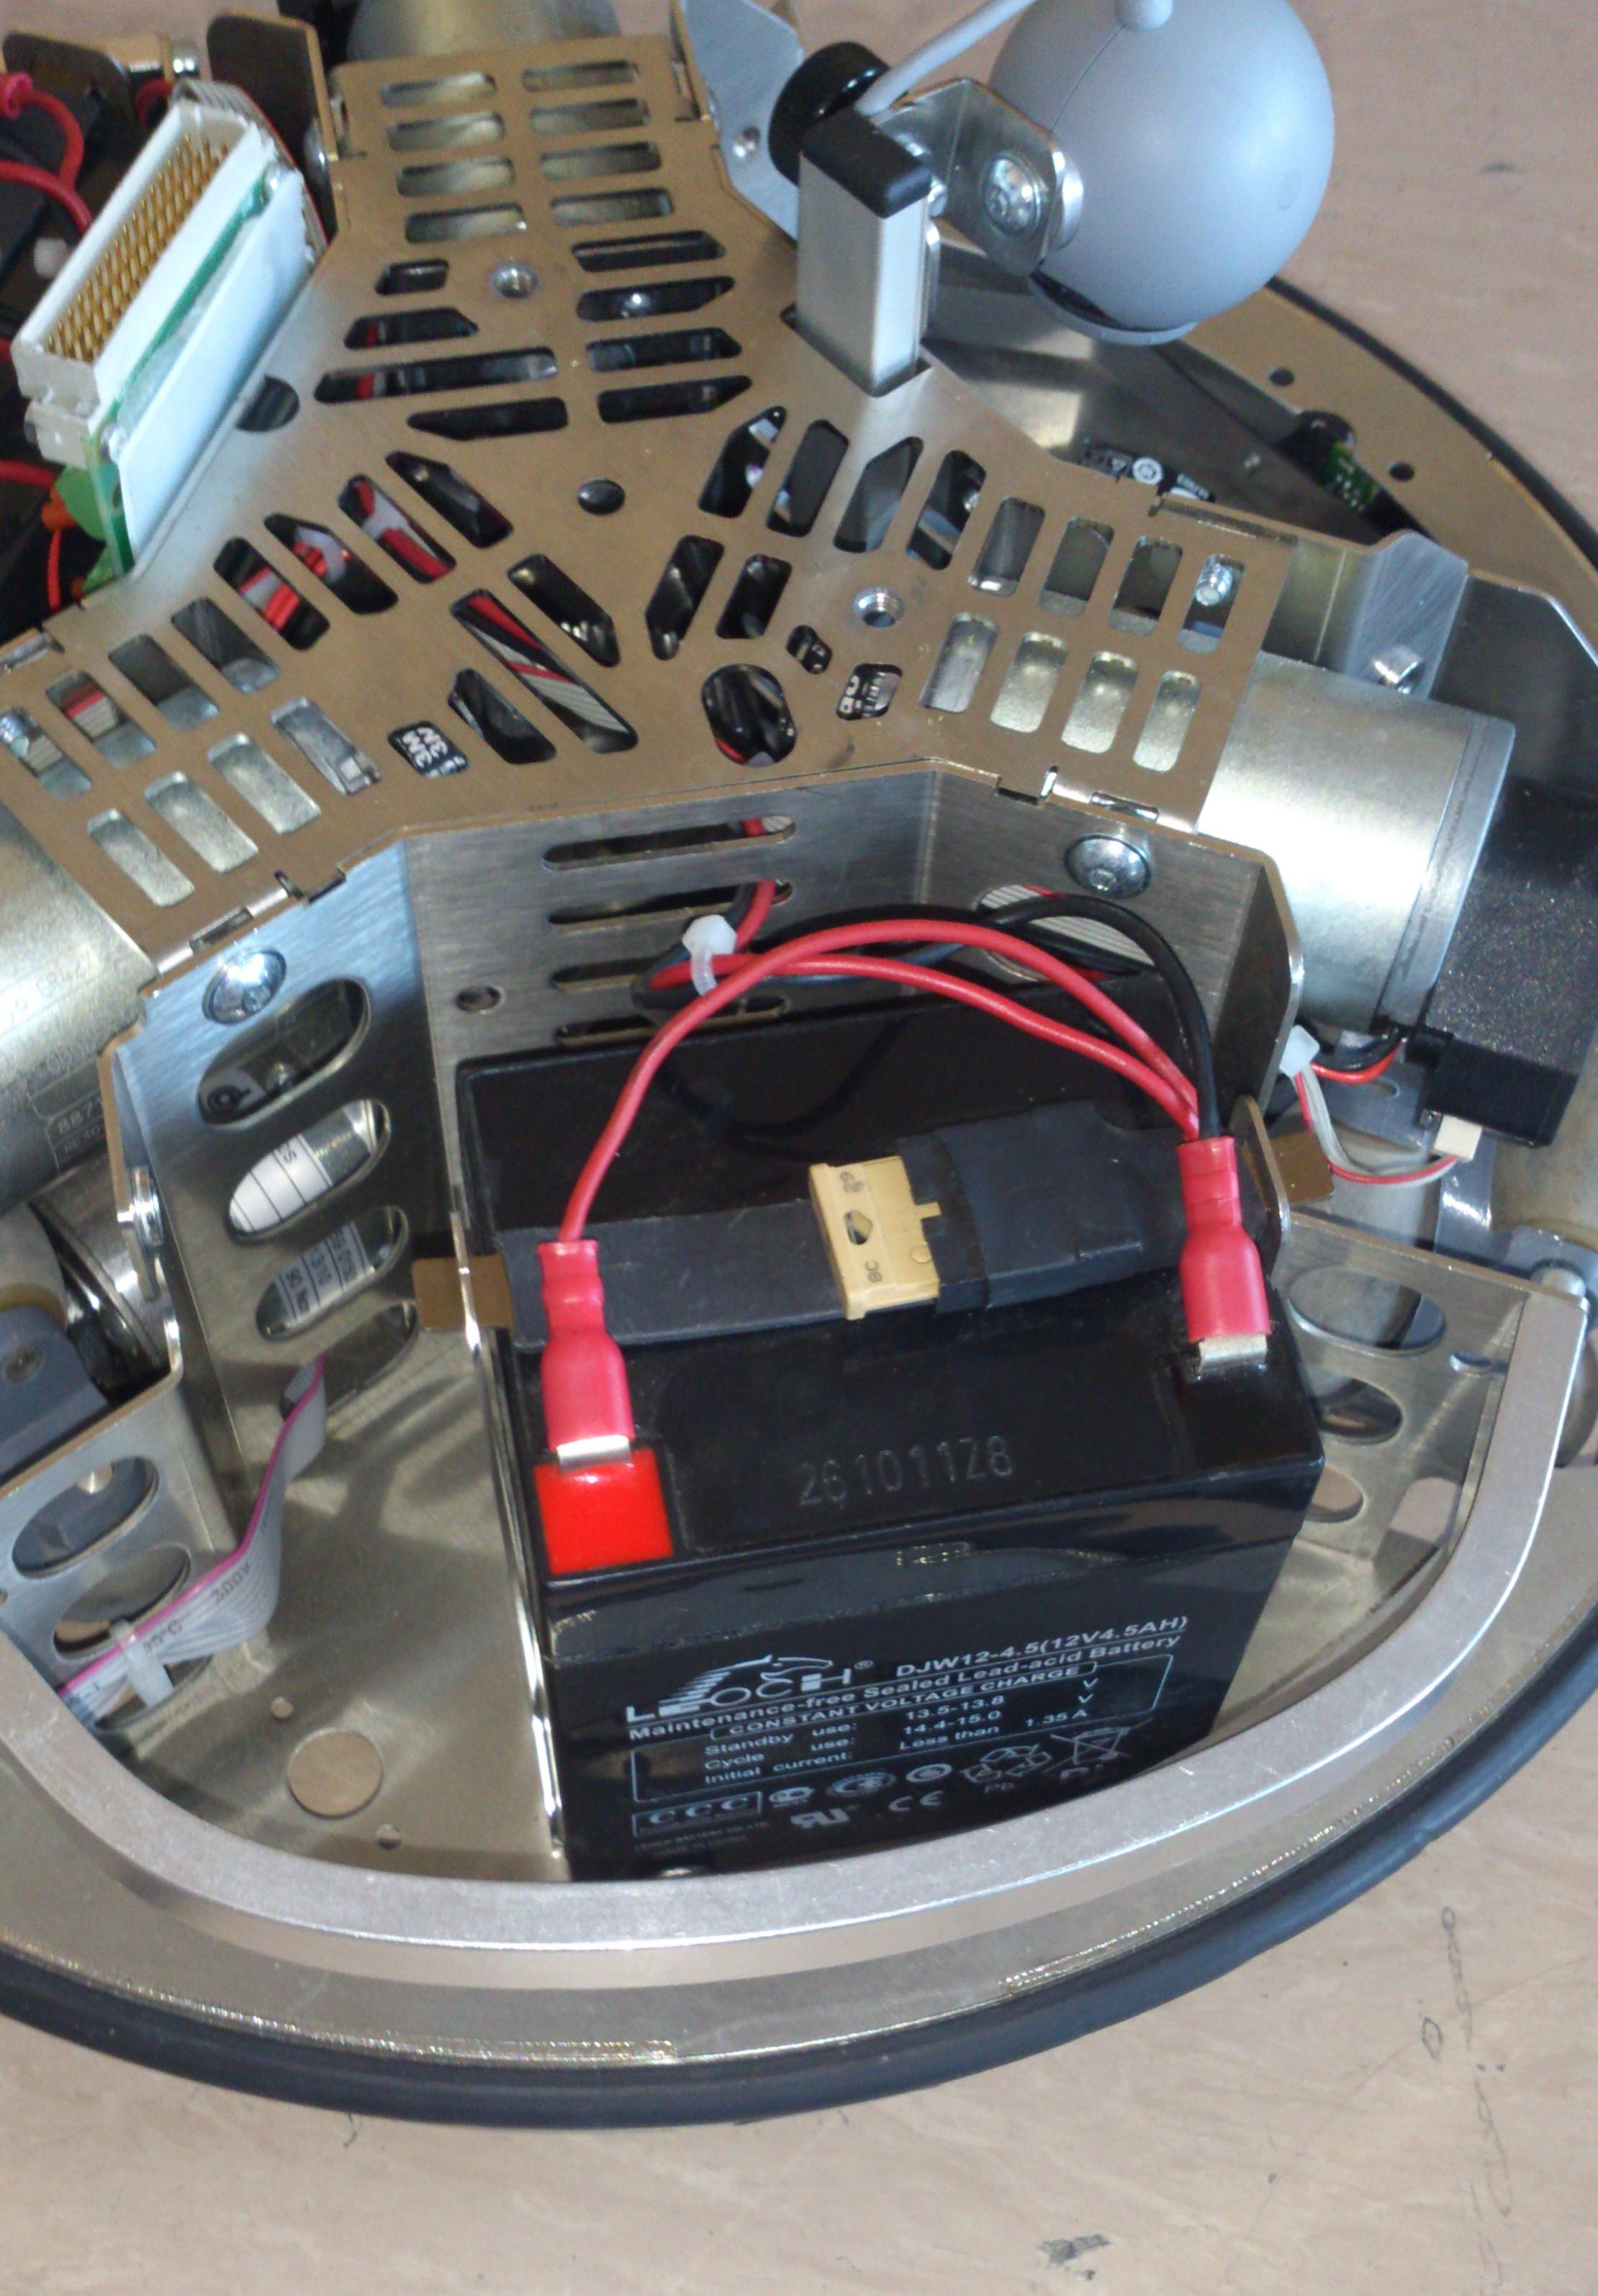
\includegraphics[height = 8cm]{remove_accum1.jpg} }
	\end{minipage}
	\hfill
	\begin{minipage}[h]{0.49\linewidth}
		\centering{ 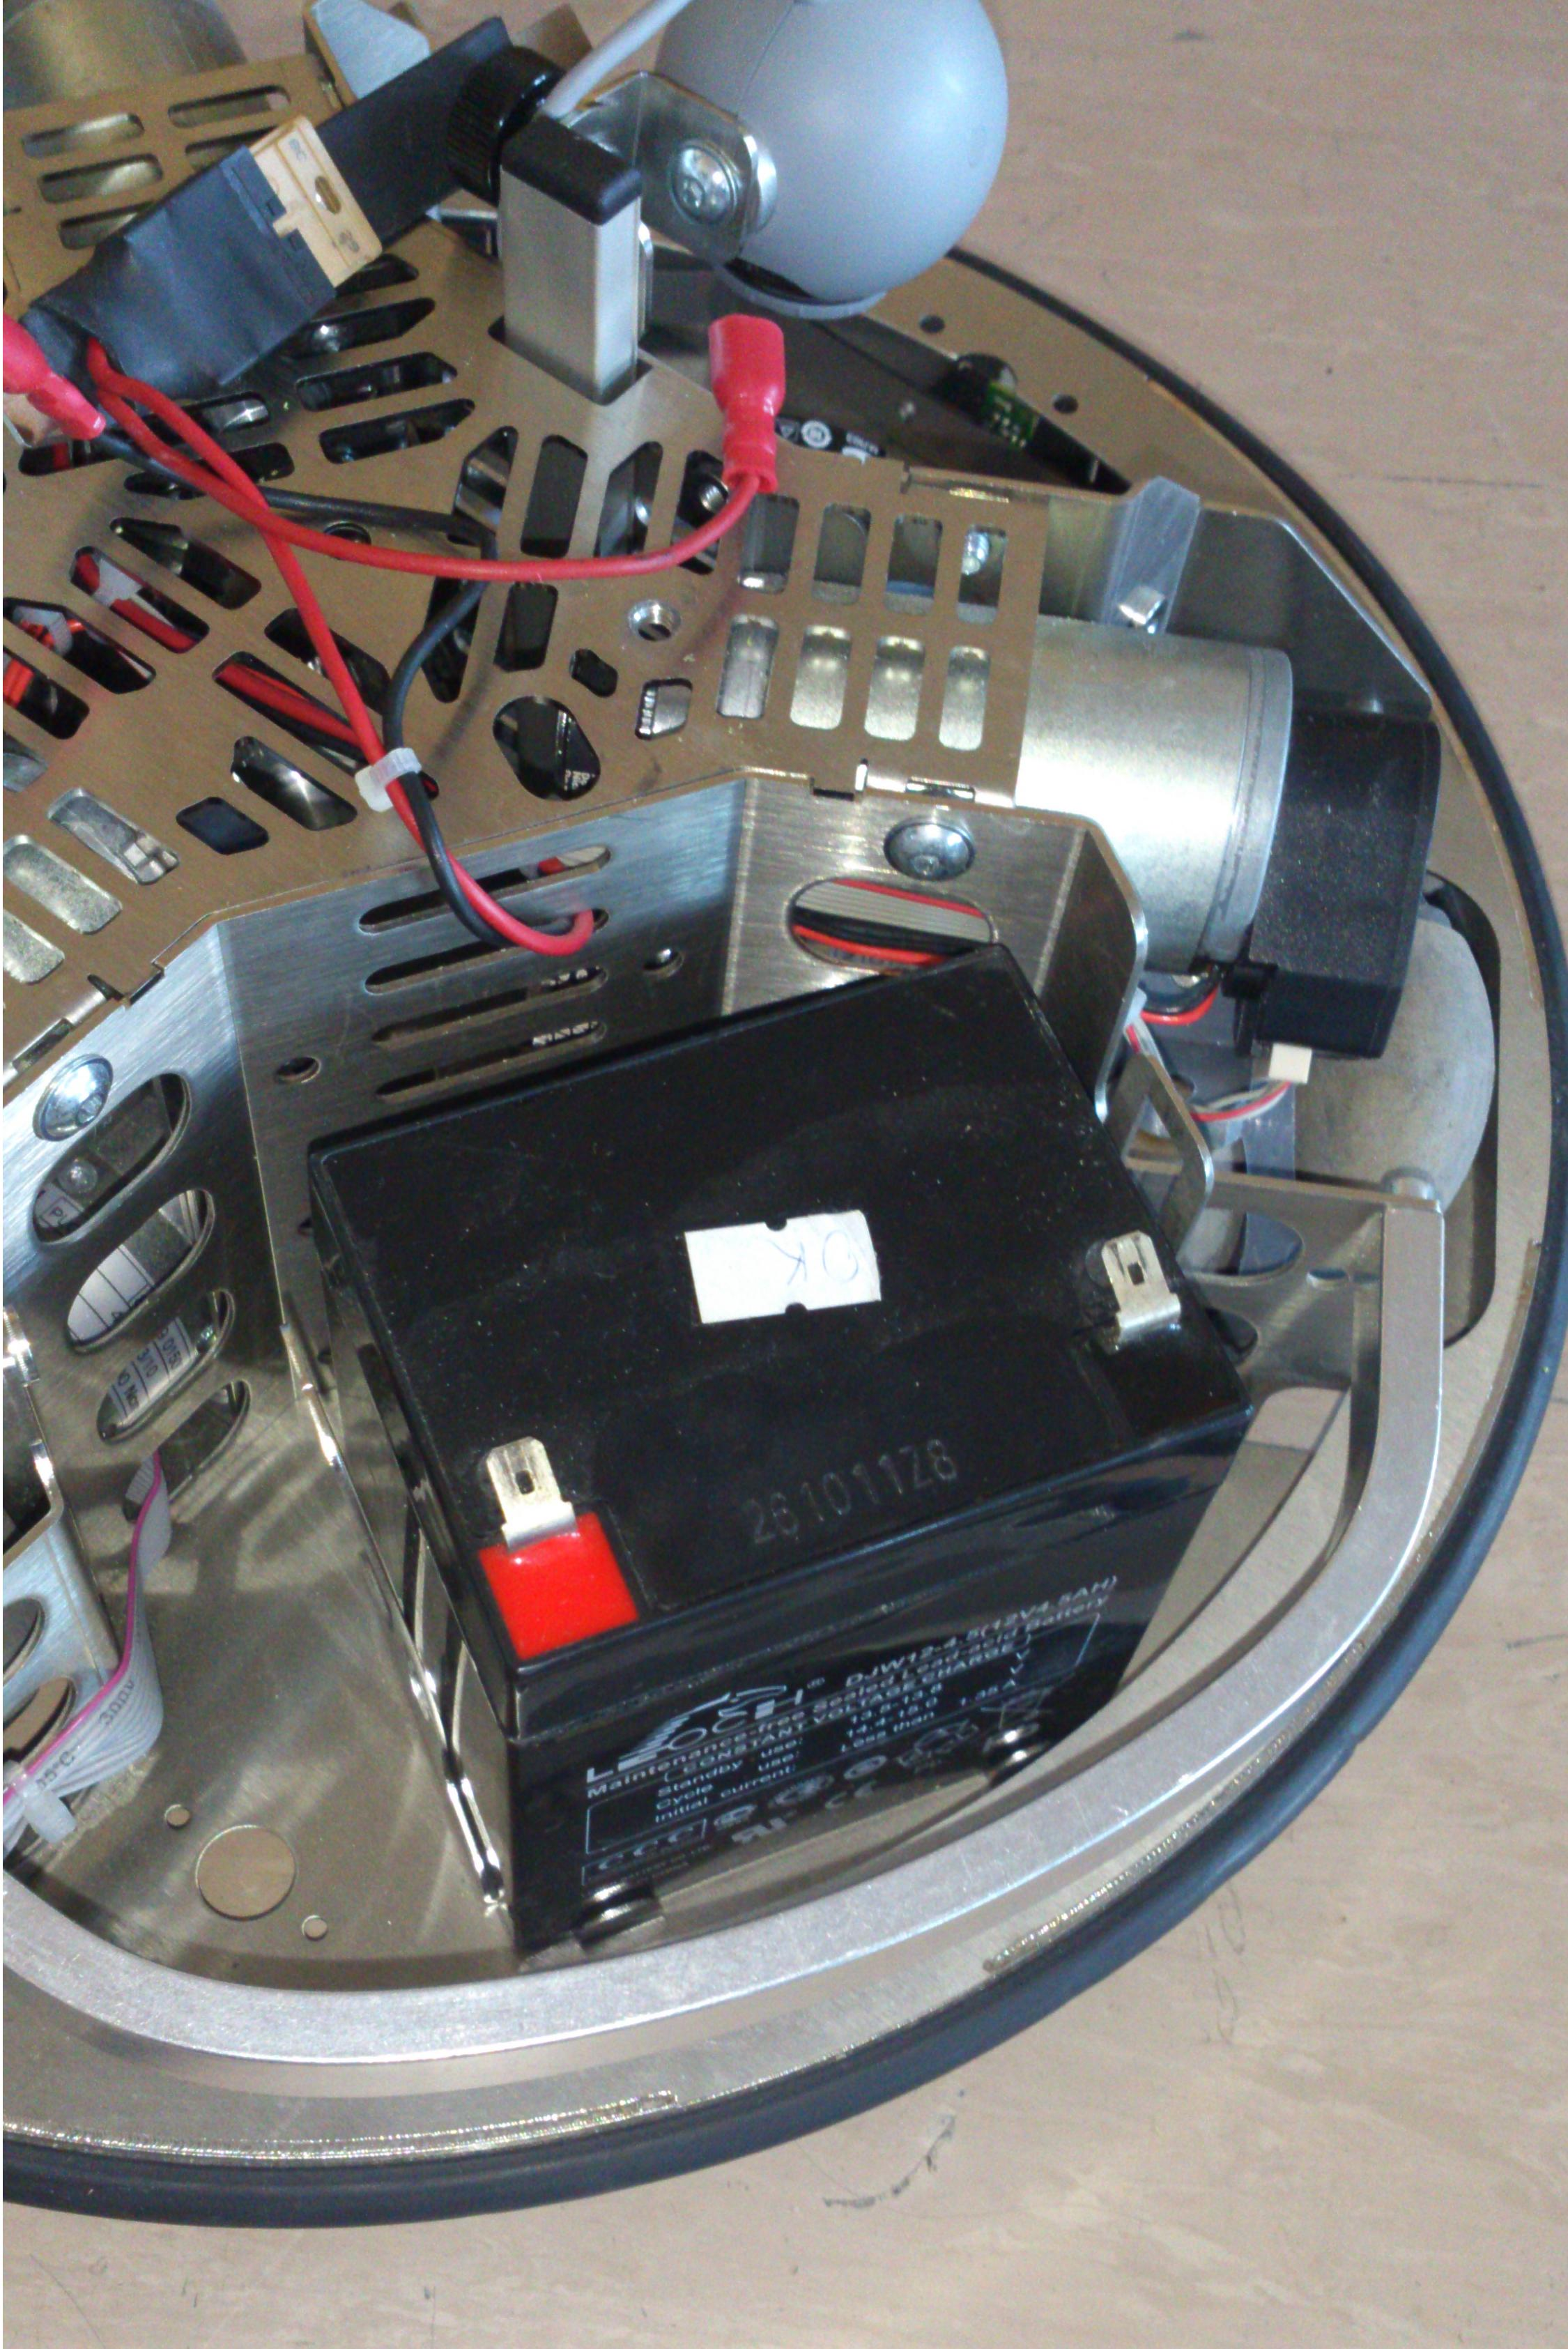
\includegraphics[height = 8cm]{remove_accum2.jpg} }
	\end{minipage}
	\caption{Отключение аккумулятора от робота.}
	\label{img_remove_accum}
\end{figure}